
%%%%%%%%%%%%%%%%%%%%%%%%%%%%%%%%%%%%%%%%%%%%%%%%%%%%%%%%%%%%%%%%%%%%%%%%%%%%%%%%%%%%%%%%%%%%%%%%%%%%%%%%%%%%%%%


\begin{figure}[h!]

\begin{center}

    \caption{Forecast and Confidence Intervals} \label{fig:Forecast1}

        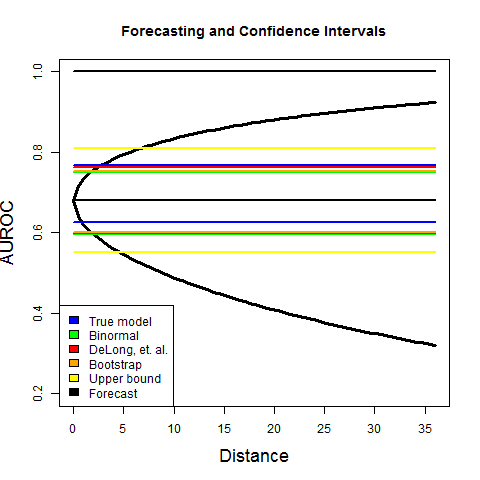
\includegraphics[scale=  0.75]{Figs/Forecast/Forecast_int_1.png}



\end{center}

    \footnotesize

        \textbf{Forecast and Confidence Intervals:}
        Forecast intervals are produced as a function of distance from the sample distribution (black curves) measured by Kullback-Leibler divergence.
        % Under the null hypothesis of a fixed sampling distribution, distance would follow a $\chi^2$ distribution with $9$ degrees of freedom.
        Confidence intervals are shown for the AUROC for a variety of methods, at the $95\%$ confidence level.
        %
        As the forecast intervals are scaled by the estimate of distance, it is possible that the intervals will expand to account for added variation, while others remain fixed.
        %
        The sample is drawn from a bi-normal distribution with a true AUROC of $0.70$, with positive classification variable distribution with a mean of $0$ and standard deviation of $1/\sqrt{2}$, and negative positive classification variable distribution with a mean of $0.5244$ and standard deviation of $1/\sqrt{2}$.
        Sample size is $1,100$ in total, with $1,000$ negative observations and $100$ positive observations.

% Terms in $KLD(\textcolor{blue}{f_1}, \textcolor{red}{f_2})
%  = \sum_{k = 1}^{K} \left\{ \textcolor{magenta}{\big( f_1(t_k) - f_2(t_k) \big)}
%         \textcolor{orange}{\log \left( \frac{f_1(t_k)}{f_2(t_k)} \right)} \right\}$

\end{figure}


%%%%%%%%%%%%%%%%%%%%%%%%%%%%%%%%%%%%%%%%%%%%%%%%%%%%%%%%%%%%%%%%%%%%%%%%%%%%%%%%%%%%%%%%%%%%%%%%%%%%%%%%%%%%%%%

